\documentclass[]{scrartcl}
\usepackage[utf8]{inputenc}
%\usepackage[upright]{fourier}
% you can change the line above
\usepackage{tkz-graph}
\usetikzlibrary{calc}
\usetikzlibrary{arrows}
\thispagestyle{empty}
\begin{document}
	
	\SetVertexNormal[Shape = circle, , LineWidth  = 1pt]
	\SetUpEdge[lw  = 1.0pt , color = black ]
	\begin{center}
		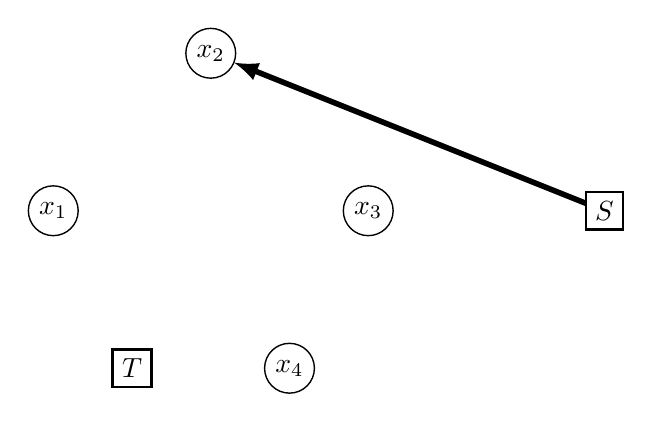
\begin{tikzpicture}
		
		\Vertex[x=1,y=-2]{$x_1$}
		\Vertex[x=3, y=0, L=$x_2$]{A}
		\Vertex[x=5 , y = -2 ]{$x_3$}
		\Vertex[x=4,y=-4 ]{$x_4$}
		
		\tikzset{VertexStyle/.style = {draw , shape = rectangle, line width = 1pt}}
		\Vertex[x=8,y=-2,L=$S$]{S}
		\Vertex[x=2,y=-4]{$T$}
		
		\tikzset{>=latex} % Set the arrowhead type!
		\tikzset{EdgeStyle/.style = {->, thick, line width = 2pt}}
		\tikzset{LabelStyle/.style = {color = black}}
		
		\Edge(S)(A)
		%\Edges($S$,$x_2$) % !! WORKS !!
		\end{tikzpicture}
	\end{center}
\end{document}